\documentclass[a4paper]{article}
\usepackage[spanish]{babel}
\usepackage[utf8]{inputenc}
\usepackage{fancyhdr}
\usepackage{charter}   % tipografía
\usepackage{graphicx}
\usepackage{makeidx}

\usepackage{float}
\usepackage{amsmath, amsthm, amssymb}
\usepackage{amsfonts}
\usepackage{sectsty}
\usepackage{wrapfig}
\usepackage{listings} % necesario para el resaltado de sintaxis
\usepackage{caption}
\usepackage{placeins}

\usepackage{hyperref} % agrega hipervínculos en cada entrada del índice
\hypersetup{          % (en el pdf)
    colorlinks=true,
    linktoc=all,
    citecolor=black,
    filecolor=black,
    linkcolor=black,
    urlcolor=black
}

\usepackage{color} % para snippets de código coloreados
\usepackage{fancybox}  % para el sbox de los snippets de código

\definecolor{litegrey}{gray}{0.94}

% \newenvironment{sidebar}{%
% 	\begin{Sbox}\begin{minipage}{.85\textwidth}}%
% 	{\end{minipage}\end{Sbox}%
% 		\begin{center}\setlength{\fboxsep}{6pt}%
% 		\shadowbox{\TheSbox}\end{center}}
% \newenvironment{warning}{%
% 	\begin{Sbox}\begin{minipage}{.85\textwidth}\sffamily\lite\small\RaggedRight}%
% 	{\end{minipage}\end{Sbox}%
% 		\begin{center}\setlength{\fboxsep}{6pt}%
% 		\colorbox{litegrey}{\TheSbox}\end{center}}

\newenvironment{codesnippet}{%
	\begin{Sbox}\begin{minipage}{\textwidth}\sffamily\small}%
	{\end{minipage}\end{Sbox}%
		\begin{center}%
		\colorbox{litegrey}{\TheSbox}\end{center}}



\usepackage{fancyhdr}
\pagestyle{fancy}

%\renewcommand{\chaptermark}[1]{\markboth{#1}{}}
\renewcommand{\sectionmark}[1]{\markright{\thesection\ - #1}}

\fancyhf{}

\fancyhead[LO]{Sección \rightmark} % \thesection\
\fancyfoot[LO]{\small{Barañao, Confalonieri, Mignanelli}}
\fancyfoot[RO]{\thepage}
\renewcommand{\headrulewidth}{0.5pt}
\renewcommand{\footrulewidth}{0.5pt}
\setlength{\hoffset}{-0.8in}
\setlength{\textwidth}{16cm}
%\setlength{\hoffset}{-1.1cm}
%\setlength{\textwidth}{16cm}
\setlength{\headsep}{0.5cm}
\setlength{\textheight}{25cm}
\setlength{\voffset}{-0.7in}
\setlength{\headwidth}{\textwidth}
\setlength{\headheight}{13.1pt}

\renewcommand{\baselinestretch}{1.1}  % line spacing


\usepackage{underscore}
\usepackage{caratula}
\usepackage{url}
\usepackage{color}
\usepackage{clrscode3e} % necesario para el pseudocodigo (estilo Cormen)




\begin{document}

\lstset{
  language=C++,                    % (cambiar al lenguaje correspondiente)
  backgroundcolor=\color{white},   % choose the background color
  basicstyle=\footnotesize,        % size of fonts used for the code
  breaklines=true,                 % automatic line breaking only at whitespace
  captionpos=b,                    % sets the caption-position to bottom
  commentstyle=\color{red},    % comment style
  escapeinside={\%*}{*)},          % if you want to add LaTeX within your code
  keywordstyle=\color{blue},       % keyword style
  stringstyle=\color{blue},     % string literal style
}

\thispagestyle{empty}
\materia{Sistemas Operativos}
\submateria{Segundo Cuatrimestre de 2015}
\titulo{Scheduling}
%\subtitulo{Subtítulo}
\integrante{Confalonieri, Gisela Belén}{511/11}{gise_5291@yahoo.com.ar} % por cada integrante (apellido, nombre) (n° libreta) (e-mail)
\integrante{Mignanelli, Alejandro Rubén}{609/11}{minga_titere@hotmail.com} 
\integrante{Sabarros, Ian}{661/11}{iansden@live.com}

\maketitle
\newpage

\thispagestyle{empty}
\vfill
%\begin{abstract}
%    \vspace{0.5cm}
%	
%
%\end{abstract}

\thispagestyle{empty}
\vspace{1.5cm}
\tableofcontents
\newpage

%\normalsize
 
\newpage

%\section{Ejercicio 1}


\section{Ejercicio 1 - TaskConsola}

Se programó un tipo de tarea llamado {\tt TaskConsola}, que se ocupa de realizar {\it n} llamadas bloqueantes, cada una con una duración al azar comprendida entre los valores {\it bmin} y {\it bmax}.

\subsection{Algoritmo}

La Figura \ref{cod-tconsola} muestra el pseudocódigo de esta tarea.

\begin{figure}[!htb]
\begin{codebox}
\Procname{$\proc{TaskConsola}(n,bmin,bmax)$}
\li \For $i \leftarrow 0 .. n$
\li \Do 	$ciclos\_bloqueo \leftarrow$ valor ``random'' en $[bmin,bmax]$
\li 		bloquear durante $ciclos\_bloqueo$ ciclos
\End
\end{codebox}
\caption{Pseudocódigo TaskConsola}\label{cod-tconsola}
\end{figure}

Para el cálculo del valor ``random'' se utilizó la función {\tt rand()} provista por la librería {\tt stdlib} de C++.

\section{Ejercicio 2 - El lote de Rolando}

Se escribió un lote de tareas para simular la siguiente situación:

\begin{itemize}
	\item Correr un algoritmo que hace un uso intensivo de la CPU por 100 ciclos sin realizar llamadas bloqueantes.
	\item Escuchar una canción, que realiza 20 llamadas bloqueantes con una duración variable entre 2 y 4 ciclos.
	\item Navegar por internet, que realiza 25 llamadas bloqueantes con una duración variable entre 2 y 4 ciclos.
\end{itemize}

Estas tareas se ponen a correr en el instante 0, 1 y 2 respectivamente, y Rolando espera que ejecute11n en simultáneo.

\subsection{Pruebas}

Se ejecutó el simulador utilizando el algoritmo FCFS para 1 y 2 núcleos, con un cambio de contexto de 4 ciclos.  Las Figuras \ref{fig-rol1core} y \ref{fig-rol2core} muestran el resultado de ambas simulaciones.

\begin{figure}[!htb]
\begin{center}
  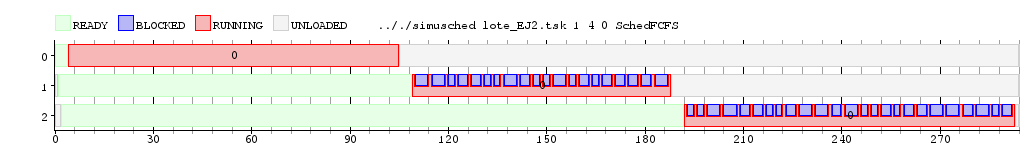
\includegraphics[scale=0.45]{imagenes/ej2-1core.png}
\end{center}
\caption{Simulación lote de Rolando con FCFS, 1 núcleo, 4 ciclos de cs}\label{fig-rol1core}
\end{figure}

\begin{figure}[!htb]
\begin{center}
  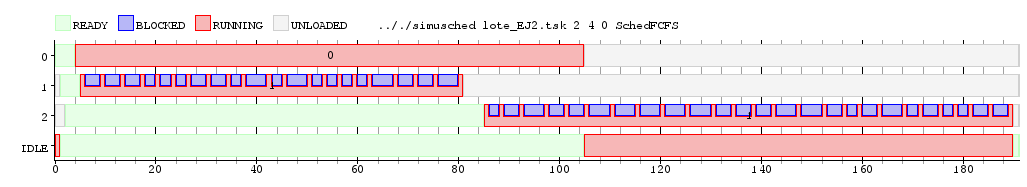
\includegraphics[scale=0.45]{imagenes/ej2-2core.png}
\end{center}
\caption{Simulación lote de Rolando con FCFS, 2 núcleos, 4 ciclos de cs}\label{fig-rol2core}
\end{figure}

En el caso de la Figura \ref{fig-rol1core}, la latencia de cada proceso es:

\begin{itemize}
	\item {\bf Tarea 0:} latencia 4
	\item {\bf Tarea 1:} latencia 108
	\item {\bf Tarea 2:} latencia 202
\end{itemize}

Estos valores nos dan un promedio aproximado de 30,3.
\vspace*{0.5cm}

Por otro lado, en el caso de la Figura \ref{fig-rol2core}, la latencia de cada proceso es:

\begin{itemize}
	\item {\bf Tarea 0:} latencia 4
	\item {\bf Tarea 1:} latencia 4
	\item {\bf Tarea 2:} latencia 83
\end{itemize}

Estos valores nos dan un promedio aproximado de 100,6.
\vspace*{0.5cm}

En el caso en el que Rolando se viera obligado a utilizar una computadora con un solo núcleo, como se utiliza un Sheduler del tipo FCFServe, no podría escuchar su canción preferida MIENTRAS corre el algoritmo, ya que las tres tareas se ejecutarán secuencialmente.  En el caso de poder utilizar una computadora con dos núcleos, podría correrse el algoritmo en uno de ellos y la canción en el otro, y Rolando podría trabajar a gusto.

\section{Ejercicio 3 - TaskBatch}

Se programó un tipo de tarea llamado {\tt TaskBatch}.  Este tipo de tarea realiza {\it cant_bloqueos} llamadas bloqueantes en momentos elegidos pseudoaleatoriamente, y cada bloqueo dura 1 ciclo.  Además, utiliza el el CPU durante {\it total_cpu} ciclos, incluyendo el tiempo necesario para lanzar las llamadas bloqueantes, pero no el tiempo en el que el proceso permanece bloqueado.

\subsection{Algoritmo}

La idea de nuestro algoritmo se basa en decidir, a cada ciclo y de manera pseudoaleatoria, si se realiza un bloqueo o no.  Para tomar esta decisión vamos a tomar un valor entero ``random'' entre 0 y 1 (1 para bloquear y 0 para no hacerlo), nuevamente utilizando la función {\tt rand()} de C++.

Como cada llamada bloqueante consume 1 ciclo de utilización de CPU, podemos decir que {\it total_cpu} incluye {\it cant_bloqueos} ciclos destinados a las llamadas bloqueantes, y el resto son usos ``puros'' de CPU.  Por este motivo, la decisión pseudoaleatoria de bloquear la tarea se realizará $total\_cpu - cant\_bloqueos$ veces. Una vez realizados todos los usos ``puros'' de CPU, sólo resta realizar las llamadas bloqueantes necesarias para completar {\it cant_bloqueos}.

La Figura \ref{cod-tbatch} muestra el pseudo-códgo de este algoritmo.

\begin{figure}[!htb]
\begin{codebox}
\Procname{$\proc{TaskBatch}(total\_cpu,cant\_bloqueos)$}
\li \For $i \leftarrow 0 .. (total\_cpu - cant\_bloqueos - 1)$
\li \Do 	$bloquear \leftarrow $ valor ``random'' en [0,1]
\li 		\If $bloquear == 1 \wedge $ aún hay bloqueos por hacer
\li 		\Then 	bloquear durante 1 ciclo
\li	 			decrementar $cant\_bloqueos$
\li 		\Else	usar CPU durante 1 ciclo
		\End
	\End
\li \While aún hay bloqueos por hacer
\li \Do 		bloquear durante 1 ciclo
\li 			decrementar $cant\_bloqueos$
	\End
\end{codebox}
\caption{Pseudocódigo TaskBatch}\label{cod-tbatch}
\end{figure}

\subsection{Pruebas}

El lote que utilizamos consta de tres tareas, las mismas tratan de mostrar el comportamiento de nuestra {\tt TaskBatch}.  Las características de estas tareas son las siguientes:

\begin{enumerate}
\item Posee sólo una llamada bloqueante, para mostrar que no siempre realizará la llamada bloqueante al final, sino que la ubicará en el medio con mayor probabilidad.
\item Posee muchas llamadas bloqueantes, de manera de que las mismas se realicen de forma consecutivas al final con mayor probabilidad.
\item Posee un número de llamadas bloqueantes cerca de un tercio de la cantidad de tiempo de cpu, para mostrar que las llamadas bloqueantes no necesariamente siguen un patrón.
\end{enumerate}

La Figura \ref{fig-batch} grafica el lote descrito utilizando un scheduler de tipo FCFS.

\begin{figure}[!htb]
\begin{center}
  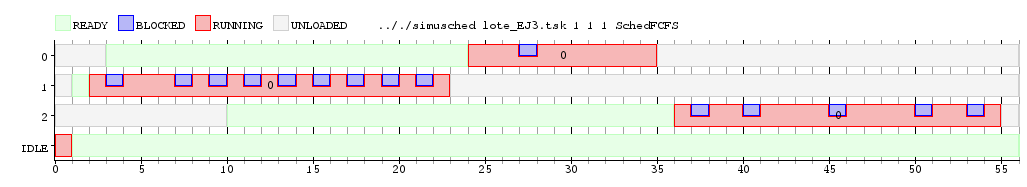
\includegraphics[scale=0.45]{imagenes/ej3.png}
\end{center}
\caption{Simulación para TaskBatch, 1 núcleo, 1 ciclo de cs}\label{fig-batch}
\end{figure}


\section{Ejercicio 4 - Round Robin}

A continuación explicaremos nuestra implementación de un Scheduler Round Robin que permite la migración entre núcleos.

\subsection{Representación}

Hemos representado las tareas con una estructura que contiene:

\begin{itemize}
\item un entero para el pid de la tarea
\item un entero para el quantum restante de la tarea, en caso de que esté en estado {\it running}
\item un booleano que indica si la tarea está bloqueada o no
\end{itemize}

Para implementar el scheduler, hemos utilizado los siguientes atributos:

\begin{itemize}
\item un arreglo de enteros de tamaño cantidad de cores utilizados, donde cada entero representa el quantum correspondiente a dicho core
\item un arreglo de tareas del mismo tamaño, donde cada tarea representa la tarea que actualmente está corriendo en dicho core
\item una lista de tareas, correspondiente a las tareas en estado {\it ready} y {\it waiting}
\end{itemize}

\subsection{Funciones}

\paragraph{Load} Se crea una nueva tarea con el pid indicado y se agrega como último elemento de la lista de tareas {\it ready} y {\it waiting}.

\paragraph{Unblock} Se recorre la lista de tareas {\it ready} y {\it waiting} hasta encontrar a la tarea con el pid indicado, y colocarla como ``no bloqueada''.

\paragraph{Tick} Se cuenta con tres casos:

\subparagraph{TICK} Primeramente se decrementa el quantum restante de la tarea actual en el cpu indicado.  Si aún tiene quantum para correr, se devuelve su pid.  En caso de que se haya terminado su quantum, se evaluará si existe otra tarea en estado {\it ready}.  De ser así, se devolverá el pid de la primer tarea que se encuentre en dicho estado en la lista de tareas.  Si no hay otra tarea para correr, sea porque todas las demás se encuentran bloqueadas o porque no existen más tareas, se devuelve el pid de la tarea actual del cpu indicado.
\subparagraph{BLOCK} Se coloca la tarea actual del cpu indicado como ``bloqueada'', se la coloca al final de la lista de tareas y se procede a buscar la siguiente tarea a ejecutar.  Si no hay más tareas o todas están bloqueadas, se devuelve la constante IDLE_TASK.  En caso contrario, se devuelve el pid de la primer tarea en estado {\it ready} que se encuentre al recorrer la lista.
\subparagraph{EXIT} Si no hay más tareas o todas están bloqueadas, se devuelve la constante IDLE_TASK.  En caso contrario, se devuelve el pid de la primer tarea en estado {\it ready} que se encuentre al recorrer la lista.


\section{Ejercicio 5}

\section{Ejercicio 6 - Round Robin vs FCFS}

Se ejecutó una simulación con el mismo lote utilizado en la sección 5, pero esta vez con un Scheduler FCFS.  La Figura \ref{fig-ej6} muestra el gráfico de dicha simulación. Los promedios de latencia, waiting-time y tiempo total de ejecución se muestran en el Cuadro \ref{tab-promedios}.

\begin{figure}[!htb]
\begin{center}
  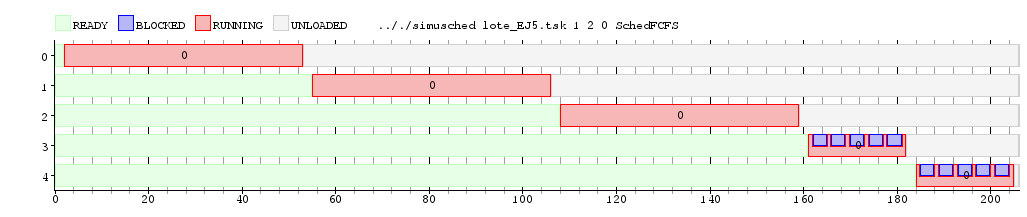
\includegraphics[scale=0.45]{imagenes/ej6.png}
\end{center}
\caption{Simulación para FCFS, 1 núcleo y 2 ciclos de cs}\label{fig-ej6}
\end{figure}

\begin{table}[!htb]
\begin{center}
\begin{tabular}{| l | l | l | l | l |}
\hline
Scheduler & Quantum & Latecia & Waiting-time & Total ejecución\\
\hline
RR & 2 & 9.8 & 208.8 & 247.8\\
\hline
RR & 10 & 24.2 & 180 & 219\\
\hline
RR & 50 & 96.2 & 141.6 & 180.6\\
\hline
FCFS & - & 102 & 102 & 141\\
\hline
\end{tabular}
\end{center}
\caption{Promedios - SchedRR y FCFS}\label{tab-promedios}
\end{table}

Podemos observar en la tabla de promedios del Cuadro \ref{tab-promedios}, que la latencia del FCFS es muy parecida a la del Round Robin con quantum 50, pero los valores de waiting-time y tiempo total de ejecución son significativamente menores. Considerando los resultados obtenidos en el ejercicio 5, podríamos concluir que de tener poca importancia, en cierto contexto de uso, el tiempo que una tarea tarda en empezar a ejecutar, utilizar FCFS tiene una mejor utilización de los recursos del cpu, dejándolo desocupado el menor tiempo posible (con las opciones con las cuales disponemos). Sin embargo, de ser prioritario el tiempo de respuesta de una tarea, sigue siendo más conveniente usar Round Robin con quantum 2.

\section{Ejercicio 7 - Scheduler No Mistery}

\subsection{SchedMistery} 

[EXPLICAR LO QUE ENTENDIMOS]

A continuación explicaremos la implementación realizada para replicar el funcionamiento del Scheduler Mistery.

\subsection{Representación}

\subsection{Funciones}

\subsection{Pruebas}

\section{Ejercicio 8 - Round Robin 2}

A continuación explicaremos nuestra implementación de un Scheduler Round Robin que no permite migración entre núcleos.

\subsection{Representación}

Para las tareas, hemos utilizado la misma estructura que en la implementación del scheduler Round Robin de la sección 4.

Para implementar el scheduler, hemos utilizado los siguientes atributos:

\begin{itemize}
\item la cantidad de cores
\item un arreglo de enteros de tamaño cantidad de cores utilizados, donde cada entero representa el quantum correspondiente a dicho core
\item un arreglo de enteros del mismo tamaño, donde cada entero representa la cantidad de tareas que están asignadas a diho core
\item un arreglo de tareas del mismo tamaño, donde cada tarea representa la tarea que actualmente está corriendo en dicho core
\item un arreglo del mismo tamaño conteniendo una lista de tareas en cada posición, donde cada lista contiene a las tareas en estado {\it ready} y {\it waiting} para cada core.
\end{itemize}

\subsection{Funciones}

\paragraph{Load} Se crea una nueva tarea con el pid indicado, se recorre el arreglo con la cantidad de tareas por cpu, y se agrega como último elemento de la lista de tareas correspondiente al cpu con menos tareas.

\paragraph{Unblock} Se recorre la lista de tareas {\it ready} y {\it waiting} de cada cpu hasta encontrar a la tarea con el pid indicado, y colocarla como ``no bloqueada''.

\paragraph{Tick} Se cuenta con tres casos:

\subparagraph{TICK} Primeramente se decrementa el quantum restante de la tarea actual en el cpu indicado.  Si aún tiene quantum para correr, se devuelve su pid.  En caso de que se haya terminado su quantum, se evaluará si existe otra tarea en estado {\it ready}.  De ser así, se devolverá el pid de la primer tarea que se encuentre en dicho estado en la lista de tareas correspondiente al cpu indicado.  Si no hay otra tarea para correr, sea porque todas las demás se encuentran bloqueadas o porque no existen más tareas, se devuelve el pid de la tarea actual del cpu indicado.
\subparagraph{BLOCK} Se coloca la tarea actual del cpu indicado como ``bloqueada'', se la coloca al final de la lista de tareas del cpu indicado y se procede a buscar la siguiente tarea a ejecutar.  Si no hay más tareas o todas están bloqueadas, se devuelve la constante IDLE_TASK.  En caso contrario, se devuelve el pid de la primer tarea en estado {\it ready} que se encuentre al recorrer la lista correspondiente.
\subparagraph{EXIT} En primer lugar, se decrementa la cantidad de tareas del cpu indicado. Si no hay más tareas o todas están bloqueadas, se devuelve la constante IDLE_TASK.  En caso contrario, se devuelve el pid de la primer tarea en estado {\it ready} que se encuentre al recorrer la lista.

\subsection{Pruebas}

\end{document}
